\section{Results}

\begin{figure*}[t]
  \centering
  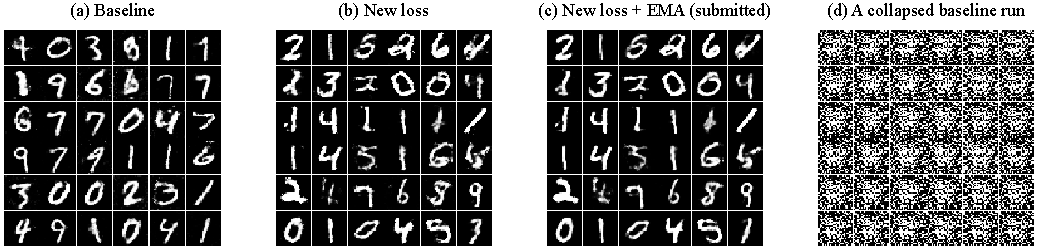
\includegraphics[width=\textwidth]{figs/combination_samples.pdf}
  \caption{Samples from the same 36 latent vectors $z$. (a) Baseline: readable digits, but many ``1''s and ``7''s and few ``2''s. (b) RpGAN + R1, raw generator: all digits appear. (c) Same run, averaged generator: cleaner strokes (submitted generator). (d) A collapsed baseline run.}
  \Description{Four grids of 6 by 6 generated digits. The baseline grid contains many ones and sevens; the RpGAN grids contain all ten digits, with smoother strokes for the averaged generator; the collapsed run outputs identical noise patterns.}
  \label{fig:samples}
\end{figure*}

\subsection{Which score should we trust?}
\label{sec:fid}
Changing the loss divides \fcnn{} by nine but leaves \finc{} unchanged (Table~\ref{tab:results}), so the two scores must see different defects. To find out which, we degraded \emph{real} test images in controlled ways (Figure~\ref{fig:fid}). \fcnn{} reacts to the balance between digits: removing one digit raises it from 2.7 to 40, and giving real images the baseline's digit proportions raises it to 124, close to the baseline's 162. \finc{} barely moves (2.4 and 7.4, for a baseline at 40). Conversely, noise on a quarter of the images is enough for \finc{} to reach the baseline's score (41) while \fcnn{} stays at 18. Digit identity explains 67\% of the variance of the classifier's features against 26\% for Inception's, in line with \cite{kynkaanniemi2023}. A direct check confirms it: resampling the baseline's images so that every digit is equally frequent lowers \fcnn{} from 162 to 32 but \emph{raises} \finc{} from 39.9 to 46.2, because the added rare digits are badly drawn.

We therefore rank models with \finc{}, which is also the platform's score and varies less between seeds (3--6\% of its value against 11--25\% for \fcnn{}), and keep \fcnn{} with the histogram of predicted digits as a diagnostic of digit balance. To see the quality of each digit, we also compute a per-digit \finc{}: our classifier sorts the generated images by digit, and 1,000 images of each digit are compared with real images of the same digit.

\begin{figure}[t]
  \centering
  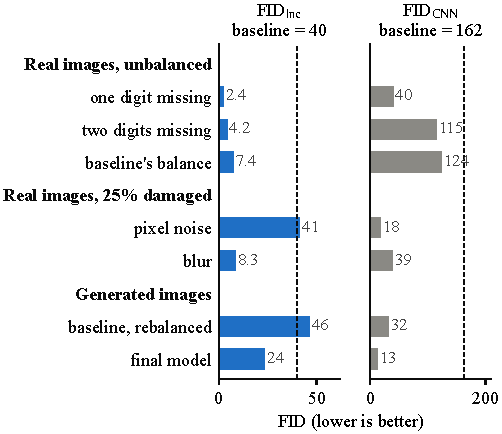
\includegraphics[width=0.82\columnwidth]{figs/fid_sensitivity.pdf}
  \caption{Both FIDs on deliberately damaged \emph{real} test images (10,000 images). Dashed lines: scores of the baseline GAN. Undamaged real images score 1.5 (\finc{}) and 2.7 (\fcnn{}).}
  \Description{Two horizontal bar charts. Missing digits and the baseline's digit balance give large FID-CNN values but small Inception FID values; pixel noise on a quarter of the images gives an Inception FID of 41, as high as the baseline, but a small FID-CNN.}
  \label{fig:fid}
\end{figure}

\subsection{Data lever}
\label{sec:data}
% Sources: data/nico_data_test.csv (selection, data protocol, runs with classifier recall >= 0.01),
% data/juliet2_test.csv (baseline loss + EMA +- noise 0.3), data/comparison_local.csv (RpGAN + R1 + EMA +- noise 0.3).
\begin{table}[t]
\centering
\small
\setlength{\tabcolsep}{4pt}
\caption{Data lever: \finc{} (mean $\pm$ s.d.\ over non-collapsed runs), precision and recall. Collapsed runs are counted separately.}
\label{tab:data}
\begin{tabular}{lcccc}
\toprule
Variant & Collapsed & \finc{} & Prec. & Rec.\\
\midrule
\multicolumn{5}{l}{\emph{Instance selection (data protocol, no EMA)}}\\
All images (reference) & 3/8 & $35.4\pm0.9$ & 0.51 & 0.52\\
Keep 95\% & 2/5 & $38.2\pm2.7$ & 0.49 & 0.48\\
Keep 90\% & 2/5 & $35.8\pm3.3$ & 0.53 & 0.49\\
Keep 75\% & 0/3 & $40.8\pm3.9$ & 0.54 & 0.40\\
Keep 50\% & 4/8 & $47.8\pm2.9$ & \textbf{0.56} & 0.32\\
\midrule
\multicolumn{5}{l}{\emph{Instance noise $\sigma_0=0.3$ (common protocol, EMA)}}\\
Baseline loss & 0/3 & $30.0\pm0.2$ & 0.56 & 0.54\\
\quad + noise & 2/5 & $30.1\pm1.3$ & 0.56 & 0.54\\
RpGAN + R1 & 0/3 & $22.1\pm1.3$ & 0.59 & 0.59\\
\quad + noise & 0/3 & $21.4\pm0.6$ & \textbf{0.60} & \textbf{0.61}\\
\bottomrule
\end{tabular}
\end{table}

\paragraph{Instance selection}
No selection rate beats the reference (Table~\ref{tab:data}): keeping 90\% ties (35.8 against 35.4) and keeping 50\% is clearly worse (47.8). Precision rises from 0.51 to 0.56 but recall falls from 0.52 to 0.32: the generator draws fewer odd digits, but also fewer kinds of digits. At 50\% it no longer draws any ``0'', which is 10\% of the data. The same trade-off appears with VGG and with classifier features, so it is not an artefact of selecting and evaluating with the same classifier.

\paragraph{Instance noise}
Noise does not change \finc{} with either loss ($p=0.91$ and $p=0.46$). Nor does it prevent collapses: with the baseline loss, 2 of 5 noised runs collapsed on the common protocol, and a paired rerun of 8 seeds on the data protocol gave 1 collapse out of 8 with noise against 3 out of 8 without ($p=0.57$). In 17 of the 19 collapsed runs we inspected, $D$ gives generated images a probability below $10^{-12}$ of being real; the binary cross-entropy of the provided code then clips, $G$'s gradient vanishes and $G$ stops learning. Noise spread over all pixels does not remove the few directions that separate real from generated images, so it cannot prevent this.

\subsection{Training lever}
\label{sec:training}
% Sources: data/juliet2_test.csv (baseline loss, raw G and G_EMA of the same runs, A100),
% data/comparison_local.csv + data/juliet2_test.csv (RpGAN + R1: G_EMA and raw G of the same runs, M3),
% data/ema_summary.csv. p-values: paired t-tests over the 3 seeds (EMA rows), Welch test (loss row).
\begin{table}[t]
\centering
\small
\setlength{\tabcolsep}{6pt}
\caption{Loss $\times$ EMA, \finc{} on the common protocol (3 seeds). Each EMA effect compares the raw and averaged generators of the same runs.}
\label{tab:loss-ema}
\begin{tabular}{lcc}
\toprule
 & Baseline loss & RpGAN + R1\\
\midrule
Raw generator & $36.6\pm1.3$ & $37.7\pm1.0$\\
Averaged generator (EMA) & $30.0\pm0.2$ & $\mathbf{22.1\pm1.3}$\\
\midrule
Effect of the EMA & $-6.7$ ($p=0.01$) & $-15.6$ ($p<0.001$)\\
\bottomrule
\end{tabular}
\end{table}

Table~\ref{tab:loss-ema} isolates the two ingredients. The new loss alone does not change \finc{} (37.7 against 36.6--38.7 for the baseline, depending on the machine). The EMA alone improves the baseline from 36.6 to 30.0. Together, they reach 22.1: the EMA gains more than twice as much with the relativistic loss as with the original one ($-15.6$ against $-6.7$, $p=0.002$), and the loss improves \finc{} by 8 points once the generator is averaged ($p=0.007$).

Figure~\ref{fig:perdigit} shows what each ingredient does. The relativistic loss \emph{rebalances the digits}: the baseline draws a ``1'' in a quarter of its images and a ``2'' in fewer than 2\%, whereas RpGAN + R1 draws each digit 8--12\% of the time. It also draws hard digits better, at fixed digit: the mean per-digit \finc{} drops from 63.6 to 55.4 ($p=0.005$), and that of ``2'' from 113 to 80. The global \finc{} hides these gains because the baseline's worst digits are also its rarest, so they weigh little in its score. No RpGAN + R1 run collapsed. The EMA then \emph{cleans the strokes of every digit} (mean per-digit \finc{} 37.3, Figure~\ref{fig:samples}c), which the global score does see.

\begin{figure}[t]
  \centering
  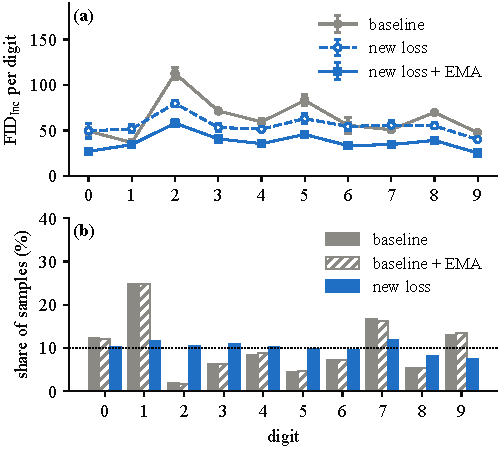
\includegraphics[width=0.86\columnwidth]{figs/training_perdigit.pdf}
  \caption{(a) Per-digit \finc{} (generated images of one digit against real images of the same digit; real data: 6.5--10.4). (b) Share of each digit among 10,000 samples; the dotted line is the balance of real data.}
  \Description{Top: per-digit FID; the baseline peaks at 113 on digit 2, the new loss lowers most digits and the averaged generator is lowest everywhere. Bottom: the baseline and baseline with EMA draw 25 percent ones and under 2 percent twos; the new loss is close to 10 percent for every digit.}
  \label{fig:perdigit}
\end{figure}

% Sources: data/comparison_local.csv (M3: baseline, RpGAN + R1 + EMA +- noise, +- DRS; one draw per seed),
% data/juliet2_test.csv (A100: baseline + EMA +- DRS, raw RpGAN + R1), data/drs_recalib_test.csv (recalibrated OBRS,
% 3 seeds x 2 draws). Submitted model: one run, platform evaluator on the MNIST test set.
\begin{table*}[t]
\centering
\small
\setlength{\tabcolsep}{5pt}
\caption{All configurations on the common protocol (200 epochs on 50,000 images, last checkpoint, 10,000 images against the MNIST test set), mean $\pm$ s.d.\ over 3 seeds. D, T, I: data, training and inference levers used. Precision and recall use VGG-16 features ($k=5$).}
\label{tab:results}
\begin{tabular}{lccccccccc}
\toprule
Configuration & D & T & I & \finc{}\,$\downarrow$ & Precision\,$\uparrow$ & Recall\,$\uparrow$ & \fcnn{}\,$\downarrow$ & Kept & Machine\\
\midrule
Baseline (provided loss) & & & & $38.7\pm1.2$ & 0.47 & 0.51 & 182 & 100\% & M3\\
\quad + DRS & & & \checkmark & $34.4\pm0.7$ & 0.51 & 0.49 & 154 & 30\% & M3\\
Baseline + EMA & & \checkmark & & $30.0\pm0.2$ & 0.56 & 0.54 & 182 & 100\% & A100\\
\quad + DRS & & \checkmark & \checkmark & $24.8\pm1.0$ & \textbf{0.62} & 0.53 & 167 & 31\% & A100\\
\midrule
RpGAN + R1, raw generator & & \checkmark & & $37.7\pm1.0$ & 0.47 & 0.47 & 19.7 & 100\% & M3\\
RpGAN + R1 + EMA & & \checkmark & & $22.1\pm1.3$ & 0.59 & 0.59 & 9.9 & 100\% & M3\\
\quad + instance noise $\sigma_0=0.3$ & \checkmark & \checkmark & & $21.4\pm0.6$ & 0.60 & \textbf{0.61} & \textbf{9.0} & 100\% & M3\\
\quad + DRS & & \checkmark & \checkmark & $22.0\pm1.1$ & 0.59 & 0.58 & 14.2 & 43\% & M3\\
\quad + OBRS, recalibrated $D$ & & \checkmark & \checkmark & $\mathbf{19.7\pm0.8}$ & \textbf{0.62} & 0.59 & 10.2 & 33\% & M3\\
\midrule
\textbf{Submitted}: RpGAN + R1 + EMA (seed 1), OBRS, recalibrated $D$ & & \checkmark & \checkmark & \textbf{19.4} & 0.61 & 0.60 & -- & 33\% & M3\\
\bottomrule
\end{tabular}
\end{table*}

\subsection{Inference lever}
\label{sec:inference}
% Source: data/drs_recalib_test.csv (A100; 3 seeds x 2 draws of 10,000 kept images each).
% Time: generation of 10,000 kept images on one A100, recalibration excluded (fitted once).
\begin{table}[t]
\centering
\small
\setlength{\tabcolsep}{3.2pt}
\caption{Rejection sampling with $D$ (3 seeds $\times$ 2 draws). AUC: probability that $D$ scores a real image above a generated one.}
\label{tab:rejection}
\begin{tabular}{lccccc}
\toprule
Filter & AUC & Kept & \finc{} & \fcnn{} & Time\\
\midrule
\multicolumn{6}{l}{\emph{Baseline}}\\
none & -- & 100\% & $38.7\pm0.8$ & 183 & 0.03\,s\\
DRS & 0.75 & 30\% & $34.3\pm0.7$ & 154 & 0.14\,s\\
OBRS & 0.75 & 33\% & $\mathbf{33.8\pm0.9}$ & 145 & 0.17\,s\\
OBRS, recalibrated & 0.83 & 33\% & $36.1\pm0.9$ & 83 & 0.16\,s\\
\midrule
\multicolumn{6}{l}{\emph{RpGAN + R1 + EMA}}\\
none & -- & 100\% & $22.0\pm1.3$ & 9.9 & 0.02\,s\\
DRS & 0.57 & 42\% & $22.1\pm1.0$ & 14.4 & 0.07\,s\\
DRS, recalibrated & 0.77 & 32\% & $20.2\pm1.1$ & 10.0 & 0.09\,s\\
OBRS, recalibrated & 0.77 & 33\% & $\mathbf{19.7\pm0.8}$ & 10.2 & 0.16\,s\\
\bottomrule
\end{tabular}
\end{table}

On the baseline, filtering works with $D$ as trained: DRS improves \finc{} from 38.7 to 34.3 and OBRS to 33.8 (Table~\ref{tab:rejection}); on the averaged baseline, DRS goes from 30.0 to 24.8. On the final model, it does nothing to \finc{} (22.0 to 22.1) and worsens \fcnn{} on every seed (9.9 to 14.4). The reason is that this $D$ can barely tell real from generated images: its AUC is 0.57, against 0.75 for the baseline's. A filter based on such a score keeps images almost at random (42\% instead of the intended 30\%), and the slight preferences it has shift the digit balance, which only \fcnn{} sees. Part of this comes from $D$ never having seen the averaged generator, but DRS also fails on the raw generator (37.7 to 38.0), so it is not the whole story.

Recalibrating $D$'s last layer raises its AUC to 0.77, and both filters then help on every seed: DRS reaches 20.2 and OBRS 19.7 ($p=0.02$, paired over seeds), with a higher precision (0.62) and the same recall. On the baseline, recalibration rebalances the digits (\fcnn{} 145 to 83) but loses to plain OBRS in \finc{}, for the reason of Section~\ref{sec:fid}: it replaces well-drawn ``1''s with badly drawn rare digits. The cost is about three proposals per kept image, i.e.\ 0.16\,s instead of 0.02\,s for 10,000 images on a GPU, plus one logistic regression fitted before generation.

\subsection{Combining the levers}
\label{sec:combination}
Table~\ref{tab:results} gathers all configurations. The gains do not add up: each lever's effect depends on the model it is applied to. The relativistic loss is worth 8 points only with EMA; DRS with $D$ as trained helps the baseline, with or without EMA, but not the final model; instance noise adds $-0.7$ on the final model, well below what three seeds can detect. Recalibrated OBRS is the only add-on that improves the final model.


\paragraph{Submitted model}
The generator is RpGAN + R1 ($\gamma=1$) with EMA, from the seed with the best validation score; images are drawn with OBRS ($K=3$) and the recalibrated $D$, which ships in place of the original one. With the platform's evaluator on the MNIST test set, the filter takes this generator from 21.2 to \textbf{19.4}, with precision 0.61 and recall 0.60 (baseline: 38.7, 0.47, 0.51). The platform scored the same generator without filter at 21.6, close to our 21.2.
